
\begin{figure*}[htb]
  \colorrule{grey3}{\textwidth}{1.5pt}
  \center
  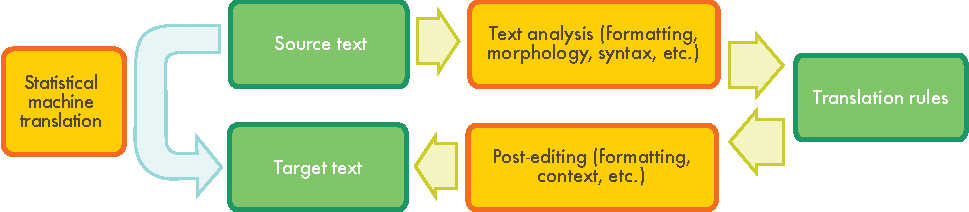
\includegraphics[width=\textwidth]{../_media/english/machine_translation}
  \caption{Machine translation (statistical; rule-based)}
  \label{fig:mtarch_en}
  \colorrule{grey3}{\textwidth}{1.5pt}
\end{figure*}

The idea of using digital computers for the translation of natural languages came up in 1946 by A. D. Booth and was followed by substantial funding for research in this area in the 1950s and beginning again in the 1980s. Nevertheless, \underbar{Machine Translation} (MT) still fails to fulfil the high expectations it gave rise to in its early years. 

At its basic level, MT simply substitutes words in one natural language with words in another. This can be useful in subject domains with a very restricted, formulaic language, e.g., weather reports. However, for a good translation of less standardised texts, larger text units (phrases, sentences, or even whole passages) need to be matched to their closest counterparts in the target language. The major difficulty here lies in the fact that human language is ambiguous, which yields challenges on multiple levels, e.g., \underbar{word sense disambiguation} on the lexical level (‘Leopard’ can mean an animal or an operating system) or the attachment of attributes on the syntactic level as in:

\begin{verse}
{\em Otcovi priatelia neprišli, moji áno.}\\
{[}Father's friends did not come, mine did.{]}\\
\smallskip
{\em Otcovi priatelia neprišli, mne áno.}\\
{[}The friends did not come to the father, {[}but{]} to me.{]}
\end{verse}

One way of approaching the task is based on linguistic rules. For translations between closely related languages, a direct translation may be feasible in cases like the example above. But often, rule-based (or knowledge-driven) systems analyse the input text and create an intermediary, symbolic representation from which the text in the target language is generated. The success of these methods is highly dependent on the availability of extensive \underbar{lexicons} with morphological, syntactic and semantic information as well as large sets of \underbar{grammar} rules carefully designed by a skilled linguist.

Beginning in the late 1980s, as computational power increased and became less expensive, more interest was shown in statistical models for MT. The parameters of these statistical models are derived from the analysis of bilingual text \underbar{corpora} such as the Europarl parallel corpus, which contains the proceedings of the European Parliament in 21 European languages. Given enough data, statistical MT works well enough to derive an approximate meaning of a foreign language text. However, unlike knowledge-driven systems, statistical (or data-driven) MT often generates ungrammatical output. On the other hand, besides the advantage that less human effort is required for grammar writing, data-driven MT can also cover particularities of the language that go missing in knowledge-driven systems, for example idiomatic expressions. 

As the strengths and weaknesses of knowledge- and data-driven MT are complementary, researchers nowadays unanimously target hybrid approaches by combining the methodologies of both. This can be done in several ways. One is to use both knowledge-driven and data-driven systems and have a selection module decide on the best output for each sentence. However, for longer sentences, no result will be perfect. A better solution is to combine the best parts of each sentence from multiple outputs, which can be fairly complex, as corresponding parts of multiple alternatives are not always obvious and need to be aligned. 

In the 1990s a prototype of MT between closely related languages was proposed for the pair Czech and Slovak at Charles University in Prague.

TEOS Trenčín markets the first practical multilingual MT software for the Slovak language, bundled with their PC dictionary software. However, since the system did not use any further linguistic analysis and simply substituted words from one language with words in the other language (mostly limited to lemmas), its usability was limited to languages that do not have much morphology – i.e. English. A later version allowed to translate webpages on the fly, a functionality that is particularly useful in the English$\rightarrow$Slovak translation, which coincidentally was the only translation direction that “worked”.

The quality of MT systems is still considered to have a huge improvement potential. Challenges include the adaptability of the language resources to a given subject domain or user area and the integration into existing workflows with term bases and translation memories. In addition, most of the current systems (not limited to the Slovak language) are English-centred. In particular, Google Translator offers the best translation quality for translations from/to English.

\boxtext{The quality of MT systems is still considered to have a huge improvement potential}

The availability of large amounts of bilingual texts is really the key in statistical MT. For Slovak, corpora of parallel texts with several other languages are currently being created. The largest data – in total several million pairs of sentences – is available in the Slovak-Czech and Slovak-English parallel corpora compiled at the Ľ. Štúr Institute of Linguistics. The corpora contain mostly fiction and are automatically sentence aligned.
